
\appendix

\section{Backup}


\begin{frame}[t]{Hyperoptimization: the reward function}
    \begin{columns}[T]
        \begin{column}{0.48\textwidth}
            \vspace{\topsep}
            Choosing as the hyperoptimization target the $\chi^2$ of fitted data results in overfitting.
        \end{column}
        \begin{column}{0.48\textwidth}
            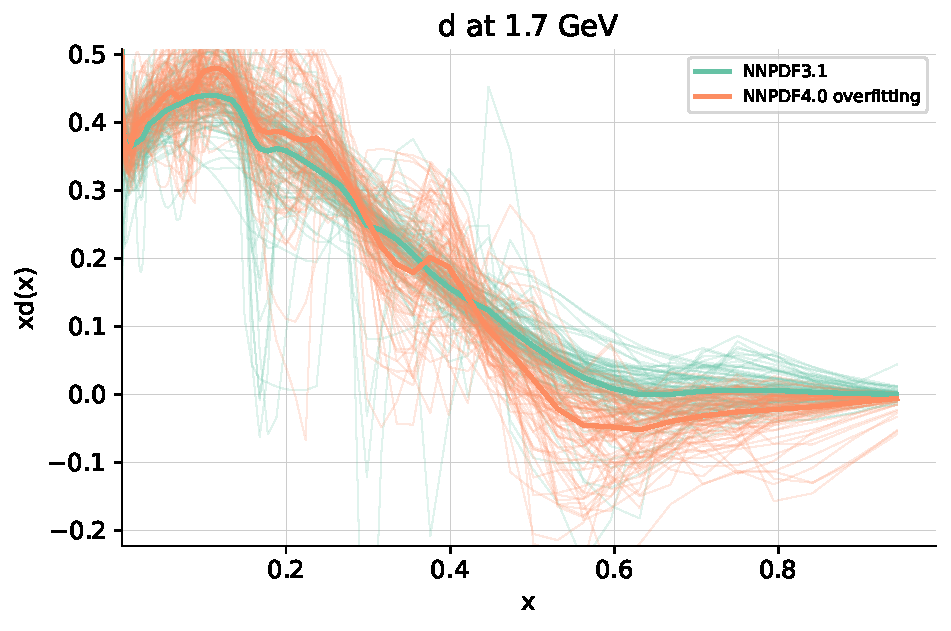
\includegraphics[width=0.9\textwidth]{overfit_nnpdf31}
        \end{column}
    \end{columns}
\end{frame}



\begin{frame}[t]{Hyperoptimization: the reward function}
    \begin{columns}[T]
        \begin{column}{0.48\textwidth}
            \vspace{\topsep}
            Choosing as the hyperoptimization target the $\chi^2$ of fitted data results in overfitting.\\
			\vspace*{2em}			
			We solve this using \textbf{k-fold cross-validation}:
			\begin{enumerate}
			    \item Divide the data into $k$ {representative subsets}
			    \item Fit $k-1$ sets and use $k$-th as test set
			    \begin{itemize}
			        \item[$\Rightarrow$] $k$ values of $\chi^2_\mathrm{test}$
			    \end{itemize}
			    \item Optimize the average $\chi^2_\mathrm{test}$ of the $k$ test sets
			\end{enumerate}
			\vspace*{0.5em}
			$\Rightarrow$ The hyperoptimization target is not based on data that entered the fit. 
        \end{column}
        \begin{column}{0.48\textwidth}
            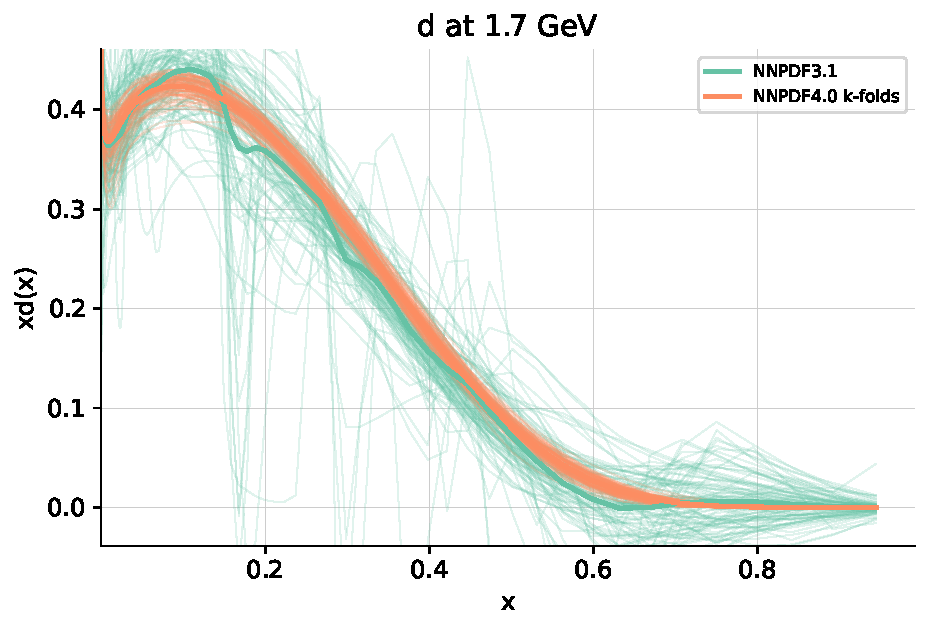
\includegraphics[width=0.9\textwidth]{best_model_vs_nnpdf31}
            \begin{itemize}
                \item No overfitting\\
			    \vspace*{0.2em}
			    \item Compared to NNPDF3.1:
			    \begin{itemize}
			        \item Increased stability
			        \item Reduced uncertainties 
			    \end{itemize}
			\end{itemize}
        \end{column}
    \end{columns}
\end{frame}